% -*- TeX:RNW:UK -*-
\documentclass[10pt]{beamer}
\usetheme{metropolis}
%\useinnertheme{rectangles}'
\setbeamercovered{%
still covered={\opaqueness<1->{15}},
again covered={\opaqueness<1->{40}}}

\hypersetup{colorlinks,linkcolor=black,urlcolor=brown,citecolor=brown}

\usepackage{amsmath,amssymb,amsthm}
\usepackage{unicode-math}

% We set the Lucida OTF fonts as default
\usepackage{fontspec}
\setmainfont{Lucida Bright OT}
\setsansfont{Lucida Sans OT}
\setmonofont{Lucida Console DK}[Scale=MatchLowercase]

\newfontfamily\typiconsfont{Typicons}[Scale=0.9]
\newcommand\typicons[1]{{\typiconsfont\symbol{#1}}}
\newcommand\Attention{\colorbox{yellow}{\textcolor{black}{\typicons{"E136}}}\xspace}
\newcommand\Advanced{\colorbox{black}{\textcolor{white}{\typicons{"E04E}}}\xspace}

\newfontfamily\webglyphsfont{WebHostingHub-Glyphs}[Scale=0.7]
\newcommand\webglyphs[1]{{\webglyphsfont\symbol{#1}}}
\newcommand\Discussion{\colorbox{white}{\textcolor{black}{\webglyphs{"F134}}}\xspace}
\newcommand\DExamples{\colorbox{black}{\textcolor{white}{\webglyphs{"F134} examples?}}}
\newcommand\Reading{\colorbox{black}{\textcolor{white}{\webglyphs{"F0C1}}}\xspace}

\newfontfamily\meteoconsfont{Meteocons}
\newcommand\meteocons[1]{{\meteoconsfont\symbol{#1}}}
\newcommand\meteosun{\meteocons{"0042}}
\newcommand\meteosuncloud{\meteocons{"0048}}
\newcommand\meteorain{\meteocons{"0052}}
\newcommand\meteosolidsun{\meteocons{"0031}}

\newfontfamily\KRfarmfont{KR Back On The Farm}
\newcommand\KRfarm[1]{{\KRfarmfont\symbol{#1}}}
\newcommand\farmplant{\KRfarm{"0049}}

\usepackage{polyglossia}
\setdefaultlanguage[variant = british, ordinalmonthday = false]{english}

\usepackage[style=authoryear-comp,firstinits,sortcites,maxcitenames=2,%
    mincitenames=1,maxbibnames=10,minbibnames=10,uniquename=mininit,%
    uniquelist=minyear,sortfirstinits=true]{biblatex}
\addbibresource{../references/ecophys.bib}
%\renewcommand{\bibfont}{\small}

\usepackage{abbrev}
\DeclareGraphicsExtensions{.png,.jpg,.jpeg,.eps,.pdf}


\title{Physiological Plant Ecology\\
       Lecture 13: Water Relations}
\author{Pedro J. Aphalo}
\date{September--October 2013}

\begin{document}


\title{PBIO-141\\Sensory and Physiological Ecology of  Plants}
\subtitle{13: Water Relations}
\author{Pedro J. Aphalo}
\date{January-February 2018}
\institute[Univ.\ of Helsinki]{M.Sc.\ in Plant Biology, University of Helsinki\\[2ex] \url{http://blogs.helsinki.fi/aphalo/}}


  \begin{frame}
    \maketitle
  \end{frame}

  \begin{frame}[c]
    \begin{center}
      \begin{small}
        \copyright 2006-2018 by Pedro J. Aphalo\\
       University of Helsinki, Finland.\\
        \textcolor{blue}{\url{http://blogs.helsinki.fi/aphalo/}}\\[2ex]
      \end{small}

      \begin{footnotesize}
        Sensory and Physiological Ecology of  Plants: `13: Water Relations' by Pedro J. Aphalo is licensed under a Creative Commons Attribution-ShareAlike 4.0 International License.

        Illustrations and text quoted from copyrighted sources is excluded from this license and their use should respect the original licenses.\\[2ex]
      \end{footnotesize}

      \centering
\includegraphics[width=6em]{../figures/copyright/by-sa}
    \end{center}
  \end{frame}

  \begin{frame}
    \frametitle{Outline}
    \tableofcontents
  \end{frame}


%\section{Stable isotopes of C}
%
%\begin{frame}{Carbon isotope ratio and $C_i$}
%    \twocolumn[lcolwidth=0.57\linewidth,rcolwidth=0.37\linewidth]{
%    \centering\includegraphics[height=0.75\textheight]{figures/Ehleringer13.7delta13CCi}}{%
%    {\small \autocite[from][]{EhlOsm1991}.}}
%\end{frame}

\section{Water and plants}

\begin{frame}{Water in plants}
    \begin{itemize}
        \item Protoplasma: 85--90\% water.
        \item Soft leaves: 80--90\% water.
        \item Ripe seeds: 10--20\% water.
        \item Life originated in the water.
        \item Conquest of land: required adaptation to dryness.
    \end{itemize}
\end{frame}

\begin{frame}{Poikilohydric plants}
    \begin{itemize}
        \item Primitive `plants' (fungi, some algae and lichens).%
        \item Mosses from dry habitats.
        \item A few vascular plants (e.g. some vascular cryptogams
        and some ferns, in the angiosperms the so called ``resurrection plants").
        \item Strategy: dehydration tolerance.
        \item Small cells, no vacuoles.
        \item Water content follows environmental fluctuations.
        \item Dryness $\rightarrow$ resting state.
        \item Wetness $\rightarrow$ active state.
    \end{itemize}
\end{frame}

\begin{frame}{Homoiohydric plants}
    \begin{itemize}
        \item Many mosses, most vascular plants.
        \item Strategy: dehydration avoidance.
        \item Big cells with big vacuoles.
        \item Cuticle and stomata.
        \item Dryness $\rightarrow$ stomatal closure.
        \item Parallel:
        \begin{description}
            \item[plants:] poikilohydric vs.\ homoiohydric.
            \item[animals:] poikilothermic vs.\ homoiothermic.
        \end{description}
    \end{itemize}
\end{frame}

\begin{frame}{Why do plants need water?}
    \begin{itemize}
        \item Biochemical and chemical reactions occur in a water
        medium.
        \item Turgor (\emph{nestej�nnitys}) or pressure is needed for cell expansion and
        structural rigidity of non-lignified organs like leaves.
        \item Photosynthesis.
        \item Transport medium.
        \item Temperature regulation (evaporative cooling).
    \end{itemize}
\end{frame}

\section{Water relations}

\begin{frame}{Movement of water}
    \begin{description}
        \item[Diffusion] No barriers. Force: difference in concentration.
        \item[Bulk flow] No barriers. Force: difference in hydrostatic pressure.
        \item[Osmosis] Semipermeable barrier or membrane. Force: water potential (result of both concentration and pressure differences).
    \end{description}
\end{frame}

\begin{frame}{Relative water content}
    Relative water content (\emph{suhteellinen vesipitoisuus}), as percent (RWC, or $R$).
    $$R = 100 \frac{M_\mathrm{f} - M_\mathrm{d}}{M_\mathrm{t} - M_\mathrm{d}}$$
    where:
    \begin{description}
        \item[$M_\mathrm{f}$:] fresh weight,
        \item[$M_\mathrm{d}$:] dry weight,
        \item[$M_\mathrm{t}$:] (full-)turgor weight. (Fully hydrated weight.)
    \end{description}
    $R$ gives the actual water content relative to the maximum water
    content of the tissue.
\end{frame}

\begin{frame}{Water potential}
    \begin{itemize}
        \item Water potential (\Wpot) is a way to specify the different kinds of forces acting on water in the soil, in the plant, and in the atmosphere.
        \item Allows to express forces in the same units, which is convenient.
        \item It is derived from the chemical potential of water:
        $$\Wpot = \frac{\mu_\mathrm{w} - \mu_\mathrm{w}^0}{\overline{V}_\mathrm{w}^0}$$
        where $\mu$ is chemical potential and $\overline{V}_\mathrm{w}$ is the partial molar volume of pure water.
        \item $\mu$ has as units J mol$^{-1}$ (Joules per mole, energy per mole of substance, or work per mole of substance).  $\overline{V}_\mathrm{w}$ has as units $\mathrm{m^3\ mol^{-1}}$.
    \end{itemize}
\end{frame}

\begin{frame}{Water potential}
    \begin{itemize}
        \item The driving force for the movement of water across membranes is the
        difference in free energy.

        \item It is common to use water potential (\Wpot) (\emph{vesipotentiaali}) for expressing the free
        energy content of the water.

        \item Water potential is defined as free energy per unit volume of water.

        \item The potential of pure water at standard conditions is
        zero. ($\Wpot^0 = 0$, the zero as superscript means standard conditions: 25\textcelsius\ and atmospheric pressure)

        \item It is expressed in pressure units (MPa, mega-Pascals; 1 MPa = 10 bar).
    \end{itemize}
\end{frame}

\begin{frame}{Water potential}
    \begin{itemize}
        \item The water potential of water that is not free or pure,
        is less than zero. ($\Wpot < 0$).
        \item Water potential measures work needed.
        \item Units: work volume$^{-1}$ (= energy volume$^{-1}$) which is equivalent to pressure.
        \item $\mathrm{J\ m^{-3} = N\ m\ m^{-3} = N\ m^{-2} = Pa}$
        \item N: Newton, Pa: Pascal, J: Joule (all SI units).
    \end{itemize}
\end{frame}

\begin{frame}{Water potential}
    The water potential (\Wpot) of a cell is given by
    $$\Wpot = \wpot[s] + \wpot[m] + \wpot[p]$$
    where \wpot[s] is the solute potential, \wpot[m] is the matric
    potential and \wpot[p] is the pressure potential.

    In tall trees, of more than 10 m, then another component becomes
    significant: gravitational potential (\wpot[g]) and must be added to the above equation.
\end{frame}

\begin{frame}{Water potential}
    $$\Wpot = \wpot[s] + \wpot[m] + \wpot[p]$$
    \begin{description}
        \item[$\bullet$] Their origin is what makes these components different.
        \item[\protect{\wpot[s]}] The solute or osmotic potential. Depends
        on the ions, and undissociated molecules in solution.
        \item[\protect{\wpot[m]}] The matric potential. Depends on
        colloidal particles or surface interactions, for example
        soils and cell walls.
        \item[\protect{\wpot[p]}] In a compartment of restricted volume,
        or almost fixed volume it counterbalances the other
        components.
    \end{description}
\end{frame}

\begin{frame}{Equilibrium}
    $$\Wpot[apo] = \Wpot[vac] = \Wpot[cyt]$$
    Water potential is in equilibrium between apoplast, vacuole, and
    cytoplasm.
    \begin{itemize}
        \item The components are different.

        \item In the vacuole \wpot[s] and \wpot[p] predominate.

        \item In the cytoplasm \wpot[m] predominates because of colloidal particles.

        \item In the apoplast (cell wall) \wpot[m] predominates because of surface
        interactions.
    \end{itemize}
\end{frame}

\begin{frame}{Water potential changes}
    \centering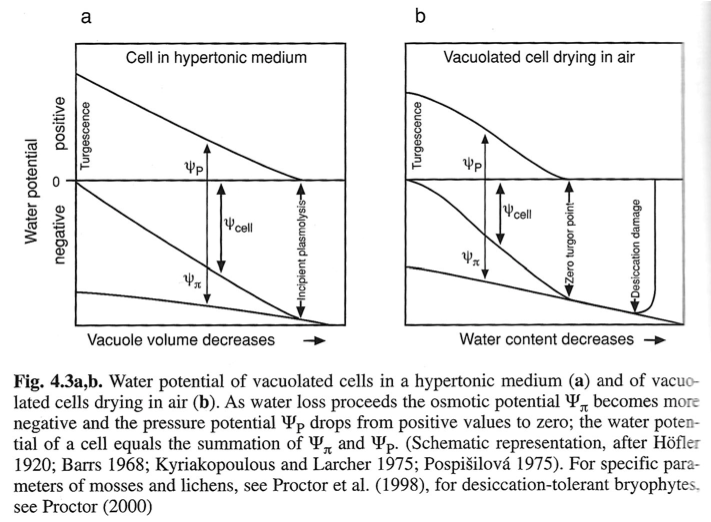
\includegraphics[height=0.8\textheight]{figures/Larcher4.3Hoffler.eps}\\
    {\small \autocite[from][]{Larcher2003}.}
\end{frame}

\begin{frame}{Movement}
    \begin{itemize}
        \item Water tends to move from regions of high water potential like soil
        and roots to regions of low water potential like leaves and the
        atmosphere. (But there are exceptions.)

        \item In the xylem the main component of \Wpot is negative pressure.

        \item In leaf cells \wpot[p] is usually positive (turgor).
    \end{itemize}
\end{frame}

\begin{frame}{Remember!}
    {\red Remember!} The driving force for water movement in the
    xylem is not the water potential, but it is hydrostatic pressure
    because it is bulk flow rather than diffusion through a
    membrane. However, the cells near the xylem vessels are at a
    similar water potential to the xylem sap because they are separated
    by a membrane.
\end{frame}

\begin{frame}{Water flow in the plant}
    \begin{itemize}
        \item Long distance movement of water in the plant occurs by bulk flow.

        \item Water in the xylem is under tension.

        \item The source of tension in the xylem is the negative pressure that
        develops in the walls of mesophyll cells when water evaporates.

        \item The cell wall acts like a very fine capillary wick soaked with
        water.

        \item Surface tension in the crevices of the wall induces a negative
        pressure in the water.

        \item Thus the motive force for xylem transport of water is generated at
        the air-water interfaces within the leaf.
    \end{itemize}
\end{frame}

\begin{frame}{Water flow out of the leaf}
    \begin{itemize}
        \item The water that evaporates from the mesophyll cell
        walls builds up the water vapour concentration in the
        intercellular spaces inside the leaf (the mesophyll air
        space).
        \item The concentration of water vapour (water vapour
        pressure, or molar fraction) is usually assumed to be saturated at
        the temperature of the leaf.
        \item Water vapour moves from the leaf interior to the atmosphere through stomata
        by diffusion.
        \item The layer of still air on the surface is called
        boundary layer, and movement of vapour through this layer is
        mostly by diffusion.
        \item The thickness of the boundary layer depends on the
        wind speed and size of the leaf.
    \end{itemize}
\end{frame}

\begin{frame}{Water path out of leaf}
   \centering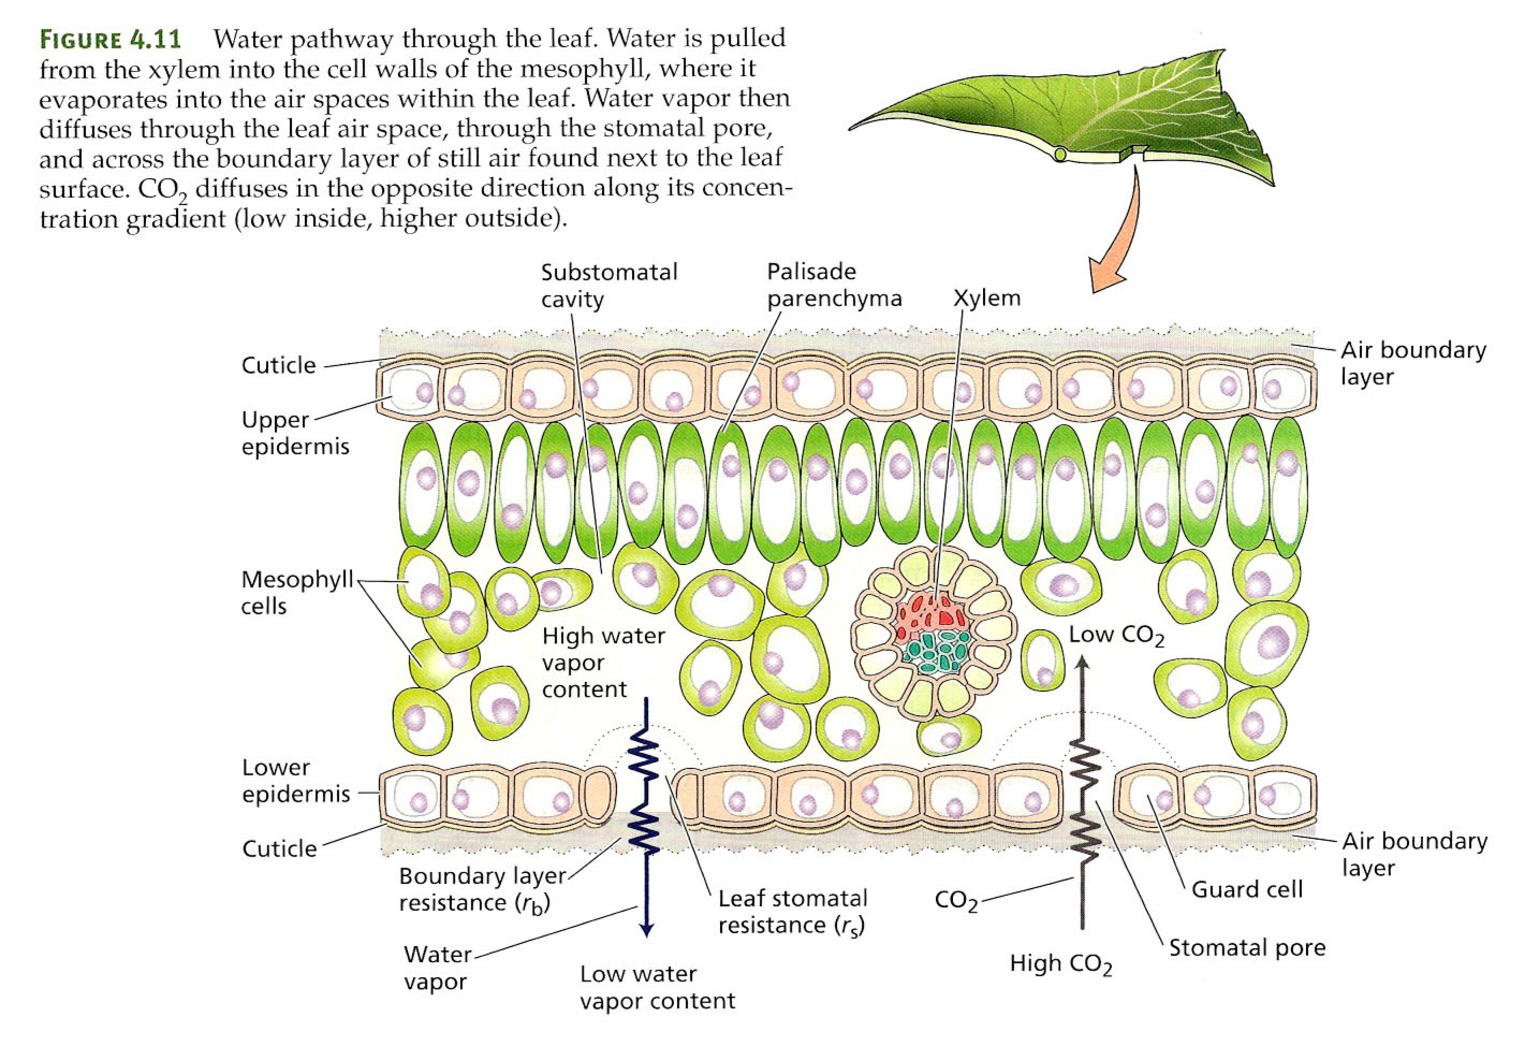
\includegraphics[height=0.85\textheight]{figures/Taiz4.11LeafCrossSection.eps}\\
    {\small \autocite[from][]{TaiZei2006}.}
\end{frame}

\begin{frame}{Stoma}
    \centering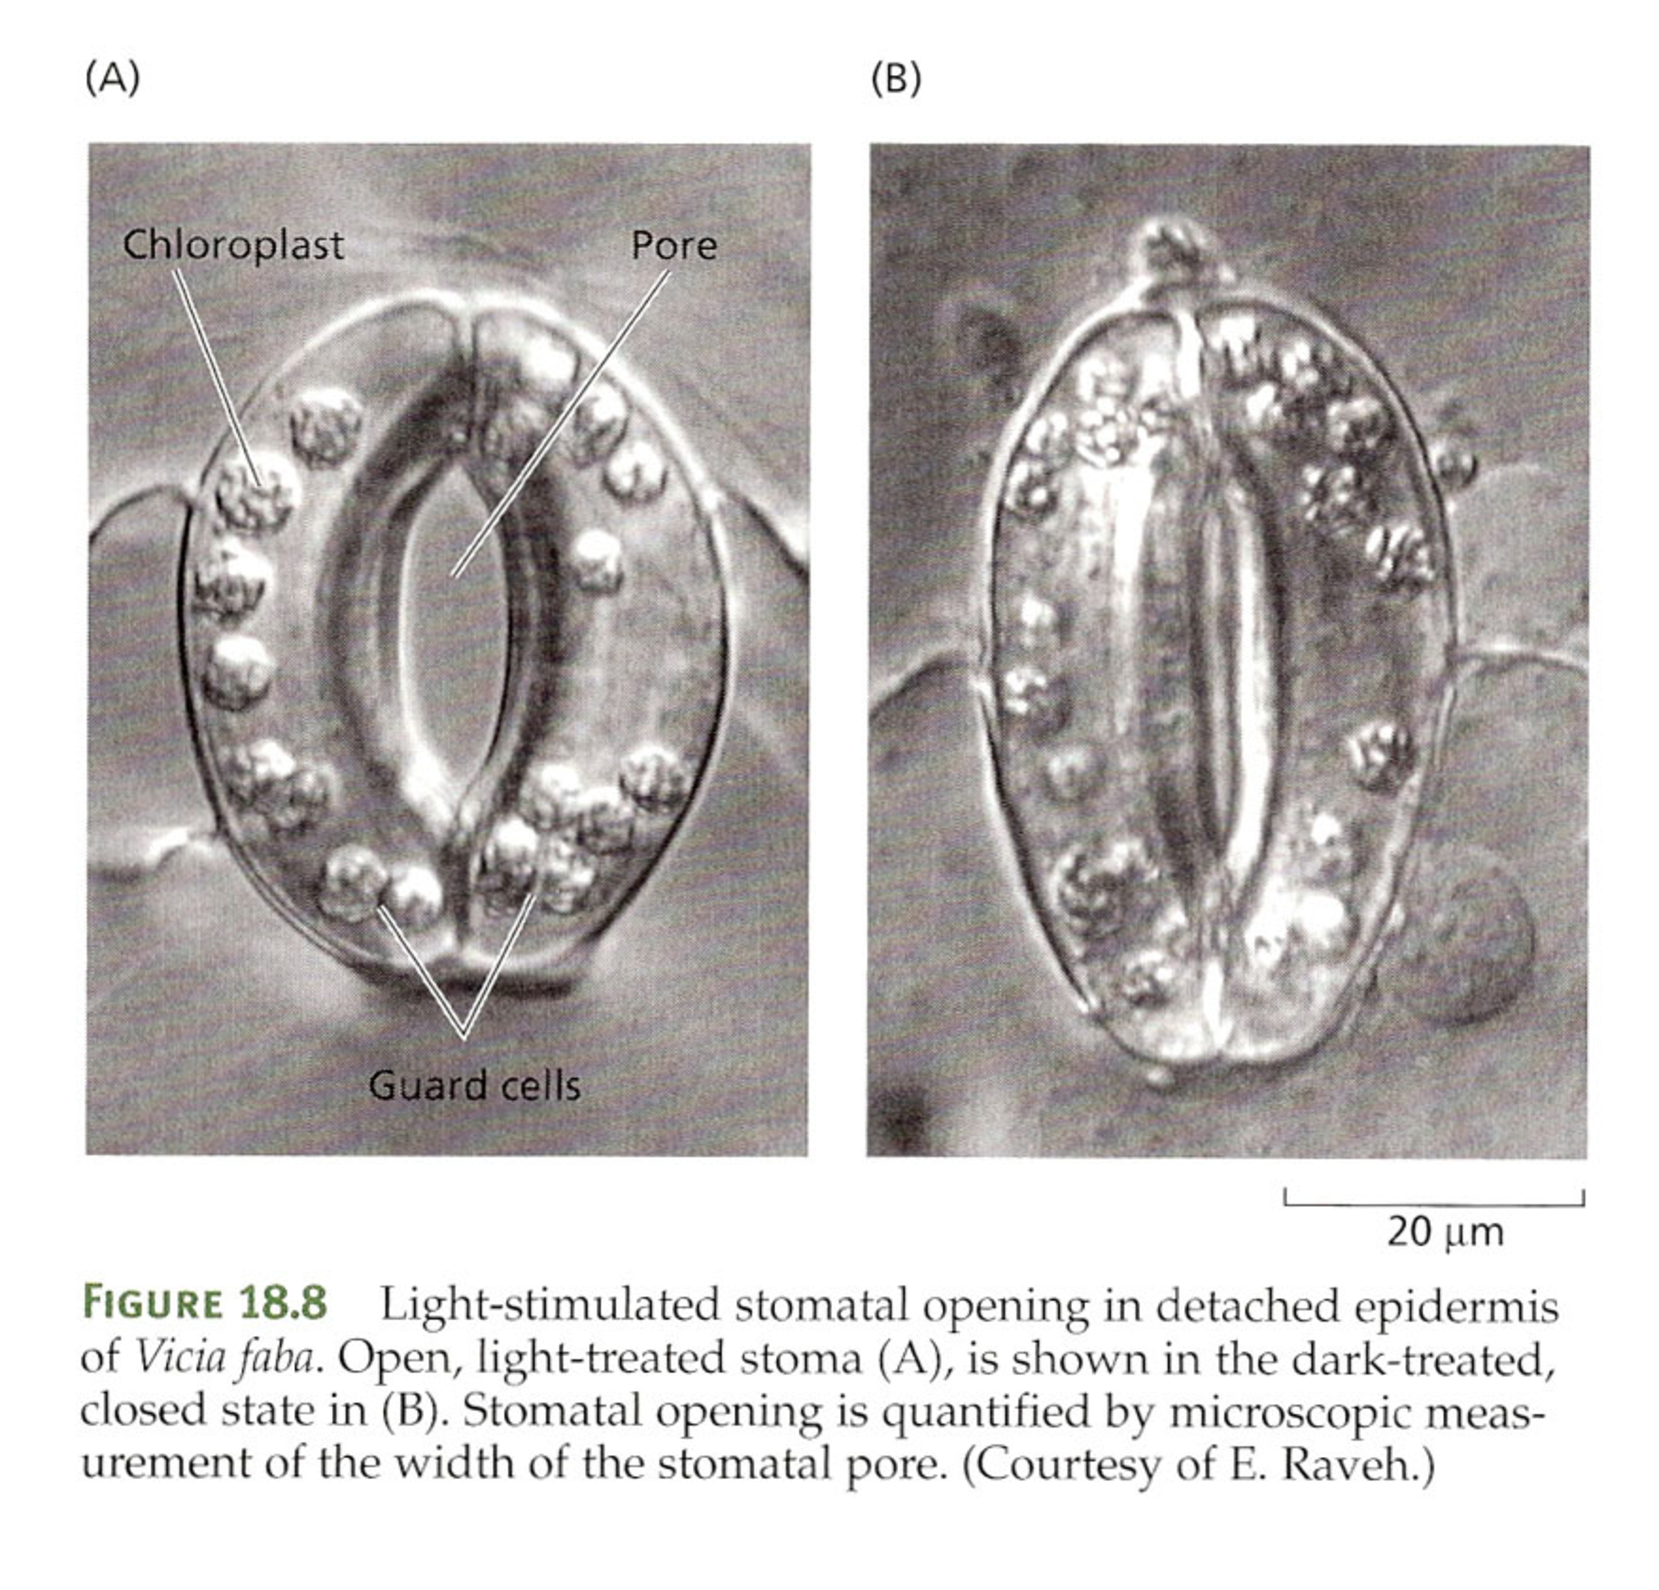
\includegraphics[height=0.85\textheight]{figures/Taiz18.8Stoma.eps}\\
    {\small \autocite[from][]{TaiZei2006}.}
\end{frame}


\begin{frame}{Water flow into the roots}
    \begin{itemize}
        \item In the roots water cannot move all the way through the
        apoplast.
        \item The Casparian bands of endodermis walls prevents it.
        \item Water must move at least part of the way through the
        symplast (the inside of the cells).
        \item Consequently the water must cross at least two
        membranes.
        \item Water movement through membranes is regulated by
        aquaporins (water permeable pores that open and close under
        metabolic control).
        \item The hydraulic conductivity is not constant.
    \end{itemize}
\end{frame}

\begin{frame}{Water path in root}
    \centering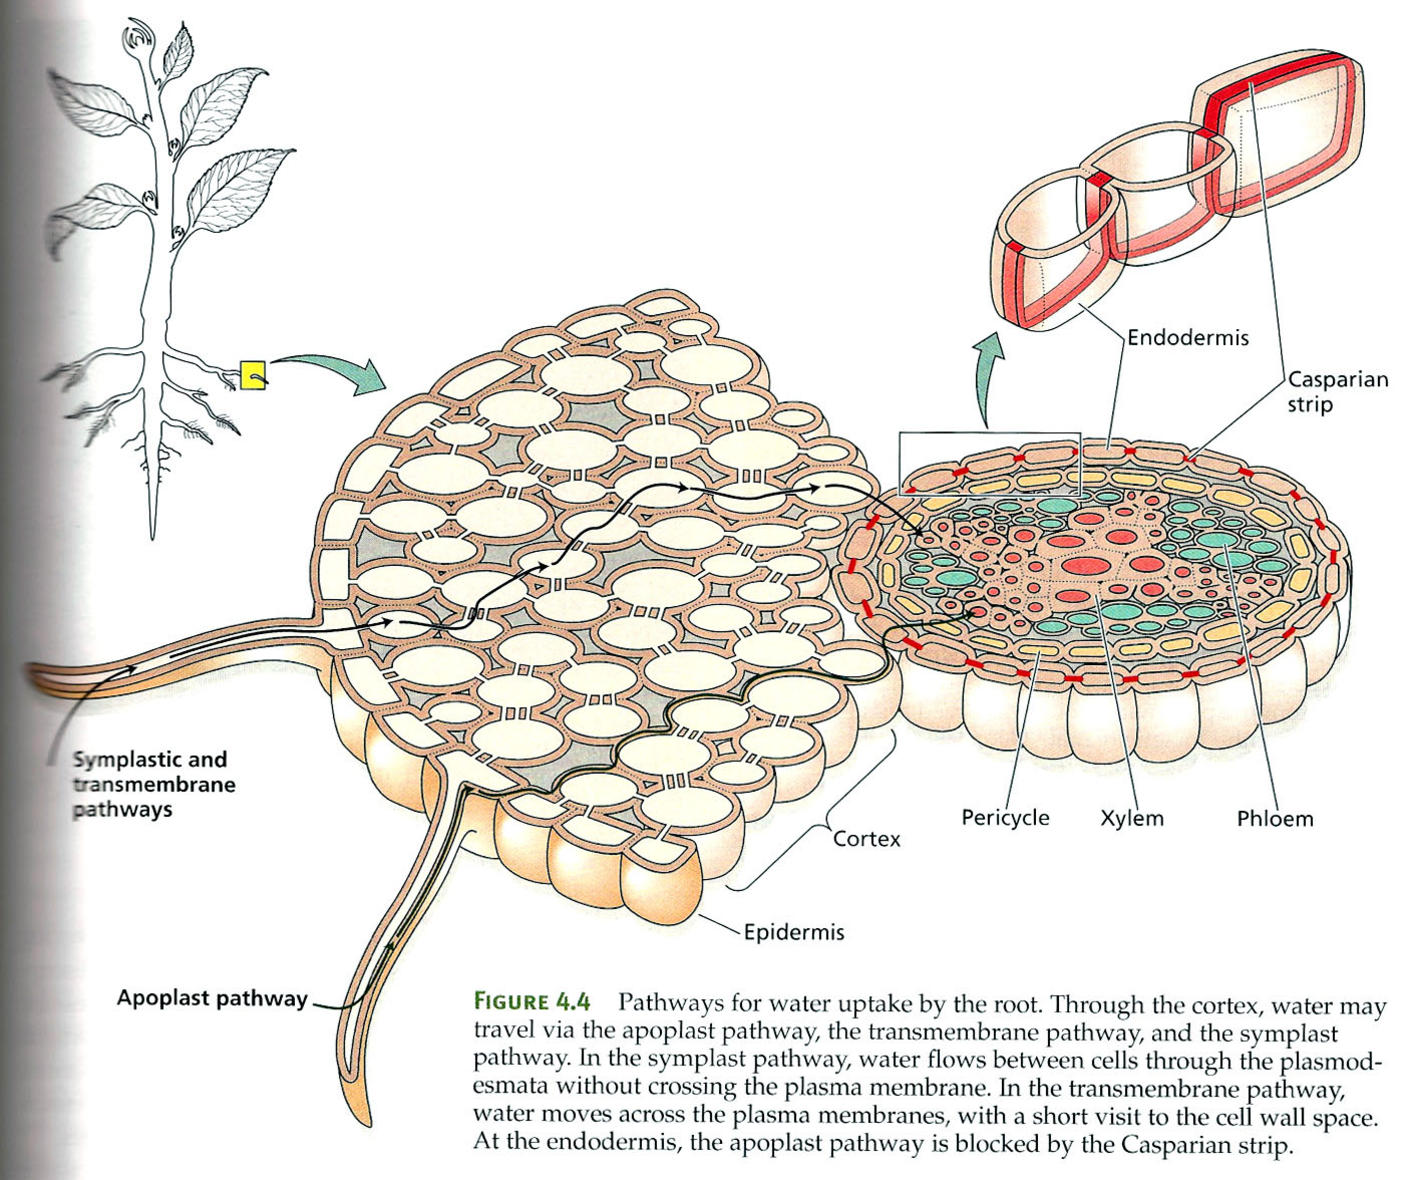
\includegraphics[height=0.85\textheight]{figures/Taiz4.4RootCrossSection.eps}\\
    {\small \autocite[from][]{TaiZei2006}.}
\end{frame}

\begin{frame}{Water path in ectomycorrhiza}
    \centering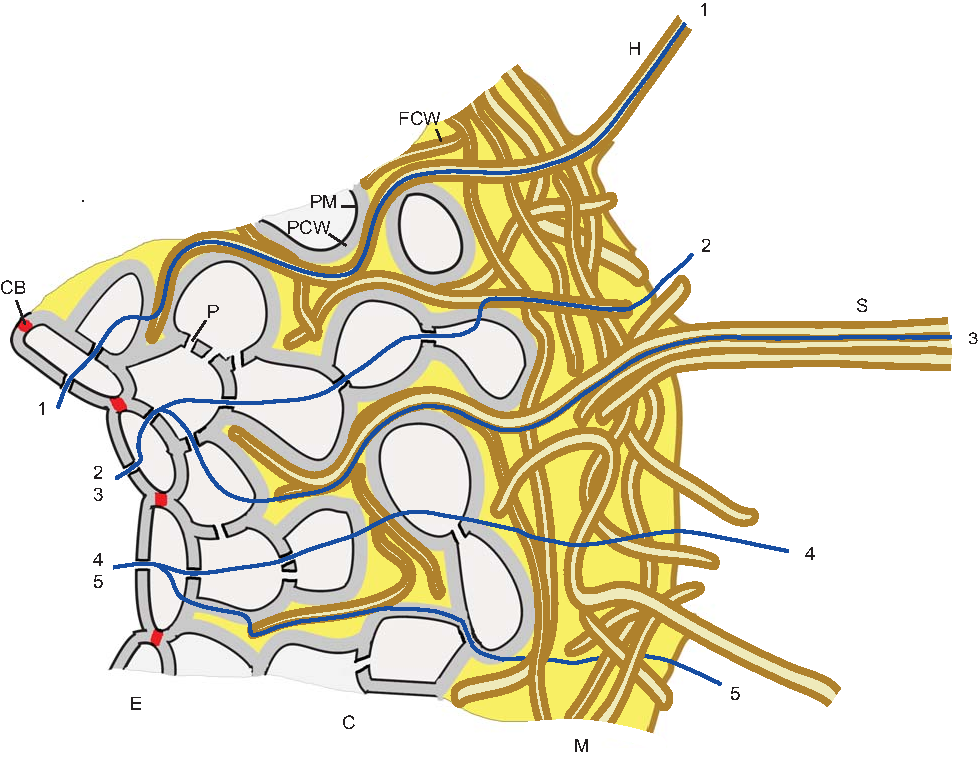
\includegraphics[height=0.85\textheight]{figures/Mykowater_Lehto.eps}\\
    {\small \autocite[from][]{Lehto2011}.}
\end{frame}


\section{Water potential in nature}

\begin{frame}{Water potential profiles}
    \begin{itemize}
        \item In transpiring plants there is a gradient in water
        potential.
        \item Highest (less negative) water potentials occur in the
        soil, and lowest water potentials usually at the top of the
        plant.
        \item At night the gradient collapses or gets very small
        because there in little transpiration.
        \item As the soil dries the water potential in the plant
        also decreases.
    \end{itemize}
\end{frame}

\begin{frame}{Water potential profiles}
    \centering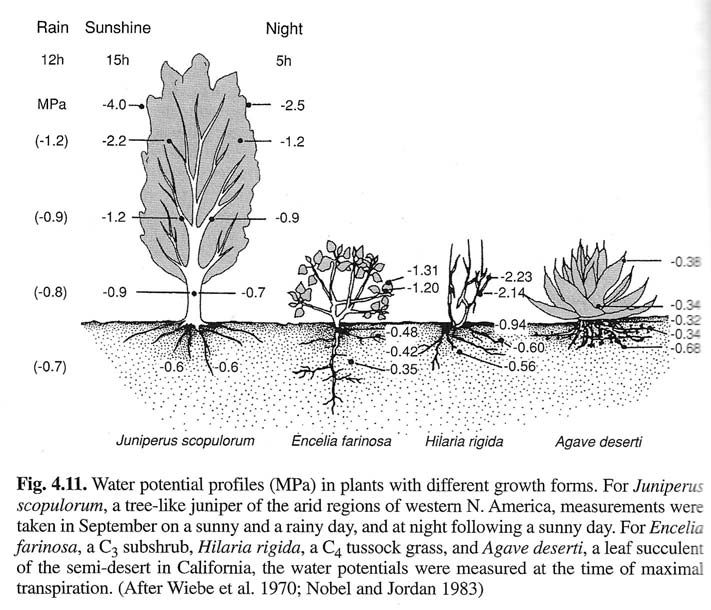
\includegraphics[height=0.85\textheight]{figures/Larcher4.11WaterPotentialProfiles.eps}\\
    {\small \autocite[from][]{Larcher2003}.}
\end{frame}

\begin{frame}{As soil dries\ldots}
    \centering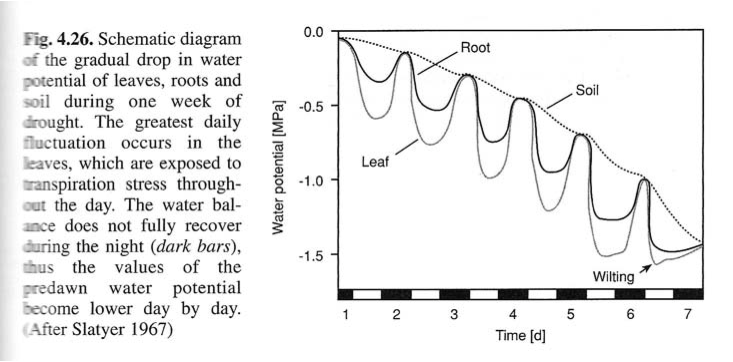
\includegraphics[width=\textwidth]{figures/Larcher4.26SchematicSlatyer.eps}\\
    {\small \autocite[from][]{Larcher2003}.}
\end{frame}

\section{Water in the soil}

\begin{frame}{Water in the soil}
    \begin{itemize}
        \item The size of pores in soils depends on the size of the soil
        particles.
        \item Sand is coarser than clay.
        \item From large size pores water drains quickly.
        \item In very small pores water is retained very tightly by
        capillary forces generating a tension (negative \wpot[p]).
        \item Water is most useful to plants if it is in medium
        sized pores.
        \item Water moves in the soil by bulk flow.
        \item Driving force in the soil is, like in the xylem, hydrostatic pressure
        (\wpot[p]).
    \end{itemize}
\end{frame}

\begin{frame}{Different soils}
    \begin{tabular}{lcc}
    \hline
    Soil       & Particle diameter & Surface area\\
               &(\textmu m)           & (m$^2$ g$^{-1}$)\\
    \hline
    Coarse sand & 2000--200        & $<$1\\
    Fine sand   & 200--20          & 1--10\\
    Silt        & 20--2            & 10--100\\
    Clay        & $<$2             & 100--1000\\
    \hline
    \end{tabular}

    {\small \autocite[adapted from][]{TaiZei2006}}

    Take into account that most soils consist in a mixture of particles of different
    sizes and may also contain organic matter (e.g. humus).
\end{frame}

\begin{frame}{Water content in soils}
    \centering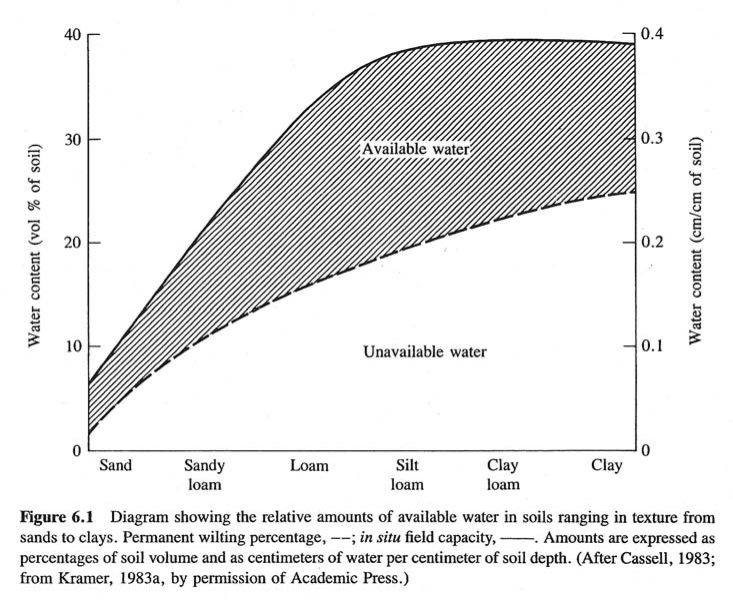
\includegraphics[height=0.8\textheight]{figures/Kozlowski6.1SoilWaterContent.eps}\\
    {\small Water available and unavailable to plants in different types of soils \autocite[from][]{Kozlowski1991}.}
\end{frame}

\begin{frame}{Water potential in soils}
    \centering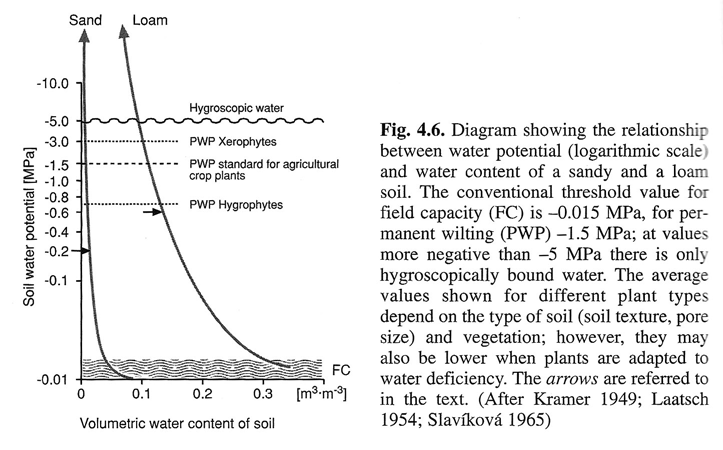
\includegraphics[height=0.75\textheight]{figures/Larcher4.6SoilWaterPotential.eps}\\
    {\small Water potential in two different types of soils \autocite[from][]{Larcher2003}.}
\end{frame}

\begin{frame}{Water uptake by roots}
    $$J_\mathrm{water} = S \frac{\Psi_\mathrm{soil} -
    \Psi_\mathrm{root}}{\sum r}$$
    where $J_\mathrm{water}$ is the flow rate (flow per unit time) of water from the soil
    into the root, $S$ is the exchange area between soil and root
    (active root surface area), \Wpot is water potential, and $\sum
    r$ the sum of all transfer resistances.
    \begin{itemize}
        \item Although the driving force is $\Delta \Wpot$, other
        factors also affect the total flow rate of water between the soil
        and the plant.
    \end{itemize}
\end{frame}

\begin{frame}{Saline soils}
    \begin{itemize}
        \item In saline soils the soil solution contains a high
        concentration of dissolved solutes.
        \item In this type of soils the solute potential (\wpot[s])
        is an important component of the soil water potential (\Wpot[soil]).
    \end{itemize}
\end{frame}

\begin{frame}{Driving forces}
    \begin{itemize}
        \item Soil water moves by bulk flow and the driving force
        is the difference in pressure ($\Delta \wpot[p]$).
        \item Through the root water moves by
        diffusion through cell membranes and the driving force is the
        difference in water potential ($\Delta \Wpot$).
        \item In the xylem water moves by bulk flow and the driving force
        is the difference in pressure ($\Delta \wpot[p]$).
        \item From the leaf air spaces to the atmosphere near the
        leaf surface water vapour moves by diffusion (but not across
        a membrane), so the driving force is the difference in
        water vapour concentration ($\Delta e$).
    \end{itemize}
\end{frame}

\begin{frame}{Driving forces}
    \centering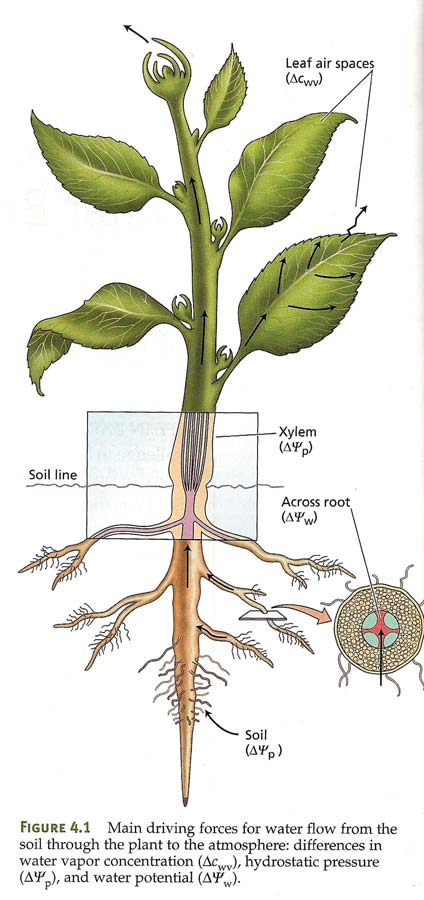
\includegraphics[height=0.8\textheight]{figures/Taiz4.1DrivingForces.eps}\\
    {\small Driving forces for water movement in different parts of
    the soil-plant-atmosphere continum
    \autocite[from][]{TaiZei2006}.}
\end{frame}

%\section{Measuring water potential}
%
%\begin{frame}{Measurements}
%    \begin{itemize}
%        \item Water potential can be measured in plant tissues.
%        \item In the xylem.
%        \item In solutions.
%        \item In the soil.
%        \item I have put in WebCT a link to a description of methods
%        for measuring water potential in plants. It is a complement
%        to the book of \citet{TaiZei2006}.
%    \end{itemize}
%\end{frame}
%
%\begin{frame}{Pressure chamber}
%    \centering\includegraphics[height=0.55\textheight]{figures/PMS1000}\\
%    {\small PMS1000 pressure `bomb' (\emph{painekammiolaite})(PMS Instruments, USA) (from \url{http://pmsinstrument.com/}).}
%\end{frame}
%
%\begin{frame}{}
%    \centering\includegraphics[height=0.8\textheight]{figures/Taiz9.2CosineLaw}\\
%    {\small .}
%\end{frame}



%\begin{frame}{Cosine law}
%    \twocolumn[lcolwidth=0.57\linewidth,rcolwidth=0.37\linewidth]{
%    \centering\includegraphics[height=0.8\textheight]{figures/Taiz9.2CosineLaw}}{%
%    \raggedright
%    {\small Irradiance on a surface depends on the angle of incidence
%    \autocite[from][]{TaiZei2006}.}}
%\end{frame}

  \section*{References}
  \begin{frame}[t,allowframebreaks]
    \frametitle{References}
    \printbibliography
  \end{frame}

\end{document}
